\chapter{Varianty simulačného modelu}

\indent\indent Vo svete okolo nástroja OMNeT++ sa za dobu od napísania našej predchádzajúcej práce venovanej simuláciám senzorových sietí udiali viaceré zmeny, ktoré nevyhnutne zasahovali aj do prípravy návrhu nášho simulačného modelu a museli byť zohľadnené. Zo všetkých týchto zmien je to posun dopredu, žiadna z nich sa neprejavila negatívne na našej práci.\\
\indent Simulačný nástroj OMNeT++ sa vyvinul do verzie 4.0, v ktorej najvýraznejšie úpravy sa dotkli jazyka NED (Network Definition Language) a datového typu premennej simulačného času \textit{SimTime}, ktorá teraz pracuje s vyšším rozlíšením. Ostatné úpravy sa veľmi nedotkli simulačného jadra, ako napríklad sú vyššia rýchlosť simulácii vo \textit{Fast} a~\textit{Express} móde pri zapnutom GUI, alebo pre fanúšikov vývojárskych IDE zahrnutie IDE Eclipse upraveného pre potreby OMNeT++ modelov (podpora NED, a pod.).\\
\indent Okrem zmien vykonaných na samotnom simulačnom nástroji sa pokrok udial aj na scéne rozšírení do OMNeT++ a objavili sa okrem novšej verzie už široko používaného rozšírenia pre bezdrôtové siete Mobility Framework (v 2.0) aj nové rozšírenia pre senzorové siete: PAWiS a MiXiM.\\

\section{Rozšírenia pre simuláciu WSN sietí}
\subsection{PAWiS}
\indent\indent Celým menom PAWiS Simulation Framework~\cite{pawis05} je rozšírenie cielené na simuláciu sietí typu WSN (Wireless Sensor Networks). Z toho dôvodu je značný dôraz kladený na správnu simuláciu správy napájania. Každá simulácia zahŕňa aj objekt \ttfamily Air\rmfamily, ktorý je obdobou modulu \ttfamily Channel Control \rmfamily z Mobility Framework. Modul \ttfamily Air \rmfamily realizuje výpočty spojené s útlmom signálu, ktorý je naviazaný na pohyb prvkov, teplotu prostredia, vibrácie zariadení, prípadne identifikuje útlm spôsobený prekážkami v priamej viditeľnosti medzi uzlami. Z praktického hľadiska funguje ako switch, do ktorého sa pripájajú všetky prvky a on následne preposiela rámce doplnené o vypočítaný útlm.\\
\indent Daný framework v podstate oproti zaužívanému Mobility Framework neponúka pre nás nič zaujímavé a nevideli sme žiadne benefity, ktoré by sme mohli využiť prechodom z MF na PAWiS. Jediná zaujímavosť v rozšírení PAWiS je uvedená správa napájania, ale tú, aj keď v jednoduchšej forme v podstate zvláda Mobility Framework doplnený o~zásuvný modul Battery plugin~\cite{forster08}.\\
\subsection{MiXiM}
\indent\indent Druhým novým produktom vo svete bezdrôtových simulácii je MiXiM. Tomuto nástroju sa povenujeme trochu hlbšie, pretože ponúka komplexnejší pohľad na simuláciu bezdrôtových sietí všeobecne. Projekt MiXiM spája v sebe vlastnosti viacerých rozšírení (okrem iného aj MF) a posúva simulačné možnosti o veľký krok ďalej.\\
\subsubsection{Vlastnosti}
\indent\indent Nástroj ponúka solídny základ pre modely a implementácie simulácii bezdrôtových sietí, vrátane modelov pre mobilné prostredia, propagáciu rádiových vĺn, podporu vo fyzickej vrstve pre modulácie a kódovania a takisto rozsiahlu knižnicu MAC protokolov a rôznych algoritmov. S čím prichádza MiXiM ako novinkou je práca s piatimi rozmermi, kde tri sú priestorové, jeden časový a piaty je frekvenčný. Vďaka tomu môžme skúmať vzájomné rušiace vplyvy rôznych kódovaní. V súvislosti so ZigBee sa vytvára vďaka nástroju MiXiM priestor pre povedzme pozorovanie vzájomného rušenia sa s nastupujúcim štandardom IEEE 802.11n (multifrekvenčný - OFDM, viacero antén - MIMO, variabilný bitrate pre hlavičku a telo správy, FEC). Modulárny dizajn pomáha pristupovať priamo aj ku komplexným situáciam a dovoľuje ľahko integrovať nové modely a implementácie protokolov. Prístup realizovaný simulátorom MiXiM je pekne popísaný v dokumente The MiXiM Vision~\cite{miximvision08}.\\
\subsubsection{Štruktúra}
\indent\indent Vlastnosti prostredia sú zahrnuté v module \ttfamily World\rmfamily . Modul \ttfamily World \rmfamily dokáže pracovať s~2-rozmerným aj 3-rozmerným priestorom (\ttfamily Playground\rmfamily). Ďalej MiXiM používa objekty, ktorými modeluje situáciu v prostredí, rôzne prekážky a podobne. Môžu to byť objekty charakteru budovy (\ttfamily ObjectHouse\rmfamily), alebo steny (\ttfamily ObjectWall\rmfamily). Tieto objekty nielen spôsobujú zmeny v šírení signálu, ale tiež kladú fyzické obmedzenia v mobilite prvkov. Správu takýchto objektov má na starosti modul nazývaný \ttfamily ObjectManager\rmfamily. Úlohu modulu \ttfamily ChannelControl \rmfamily z Mobility Framework prebral modul \ttfamily ConnectionManager\rmfamily. On dynamicky vytvára spojenia medzi uzlami tak, aby sa zbytočne nestrácal výpočtový výkon na simulovanie spojení, ktoré majú takmer nulovú váhu nielen čo sa týka kvality prenosu správ, ale aj z pohľadu príspevku k rušeniu na jednotlivých prijímačoch. Modul \ttfamily ConnectionManager \rmfamily sa vždy zaoberá výpočtom okolo jedného konkrétneho typu vlnenia. To znamená, že pre spoločnú simuláciu dvoch rôznych sietí v pásme ISM 2.4~GHz a GSM 900~MHz budeme mať v simulácii 2 moduly typu \ttfamily ConnectionManager\rmfamily.\\ 
\indent Čo sa týka samotných uzlov, aj tu je vidieť, že ľudia, ktorí stoja za projektom MiXiM majú na svedomí aj projekt Mobility Framework. Štruktúra jednotlivých modulov v komunikačných uzloch je veľmi podobná tej z Mobility Framework (bližšie o nej v~\cite{halas03}). Sprostredkovanie prenosu informácii medzi jednotlivými modulmi už sa nedeje cez modul \ttfamily Blackboard\rmfamily, ale cez modul \ttfamily Utility\rmfamily. Ich funkcie sú totožné. Ďalej pribudol modul pre sledovanie spotreby a predikciu výdrže energie \ttfamily Battery \rmfamily a modul pracujúci so smerovacími mechanizmami \ttfamily Arp\rmfamily.\\
\indent Hlavná logika frameworku je ukrytá v moduloch a rozhraniach pre posielanie správ, ich transformácie do signálovej podoby a následné spracovanie prijatého signálu aj s~informáciami o útlme a pod.
\paragraph{Signal}
\indent V simulácii signálu vstupuje u vysielacieho prvku do modelu faktor antény, prenosová rýchlosť, vysielací výkon a frekvencia (komunikačný kanál). Na prijímacej strane je výsledok ovplyvnený útlmom na prenosovom médiu, prijímacou anténou a aj útlmom spôsobeným prekážkami v linii priamej viditeľnosti, pretože, ako sme už spomenuli, práca s takýmito objektami je v istej podobe zvládnutá v simulačnom frameworku.
\paragraph{AnalogueModel}
\indent Miesto, v ktorom sú počítané uvedené faktory prijímaného signálu (útlmy, zisk antén).
\paragraph{Decider}
\indent Modul \ttfamily Decider \rmfamily rozhoduje o výslednom prijatí, alebo zahodení rámca, na základe rušenia a šumu. Aplikuje algoritmy FEC (Forward Error Correction) a tiež informuje nadradené vrstvy o stave prenosového média (busy/idle). Táto vrstva je miesto prechodu z analógového pohľadu na model na digitálny.
\paragraph{\textit{Radio}}
\indent Bod, v ktorom sú prepínané stavy rádia (\textit{RX}, \textit{TX}, \textit{IDLE}, \textit{SLEEP}). Tieto stavy sú riadené vyššími vrstvami. Prípadne modul \ttfamily Radio \rmfamily môže obsahovať premenné, ktoré definujú rýchlosť prechodu medzi stavmi (napr. RX-to-TX time).
\paragraph{ChannelInfo}
\indent Pracuje s rámcami a komunikuje s vrstvou \ttfamily BasePhyLayer \rmfamily aby mohol do rámcov doplniť údaje doplňujúce dáta vyžadované modulom \ttfamily Decider\rmfamily. Dopĺňa rámce vypočítanými hodnotami premenných RSSI (Received Signal Strength Indication) a~SINR (Signal to Interference plus Noise Ratio).
\paragraph{BasePhyLayer}
\indent Je čisto OMNeT++ modul. Komunikuje s vyššími vrstvami cez správy, ktorých obsah je popísaný výhradne NED jazykom.\\ \\
\indent Podrobné vzťahy sú schematicky vyobrazené na obr.~\ref{fig:architecture_mixim}.\\
\begin{figure}[htbp]
\begin{center}
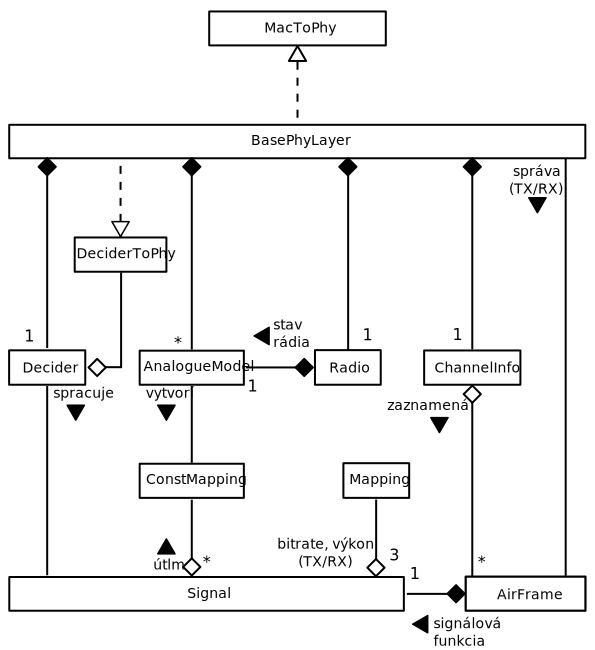
\includegraphics[width=140mm]{figures/architecture_mixim}
\caption{Práca so signálovou časťou simulácie vo frameworku MiXiM}
\label{fig:architecture_mixim}
\end{center}
\end{figure}
\subsection{Mobility Framework}
\indent\indent Mobility Framework~\cite{mf03} je overený framework pre simulovanie bezdrôtových sietí postavený ako modul do simulátora OMNeT++. Medzi jeho nesporné výhody patrí jednoduchosť, prehľadnosť a rýchlosť behu simulácii. Nakoľko vývoj rozšírenia MiXiM sa zatiaľ nedostal do použiteľného stavu, ako najvýhodnejšie sa momentálne javí zostať pri frameworku MF. Ten sa medzičasom dočkal vývojovej verzie 2.0, v ktorej zostal vývoj zakonzervovaný, adaptovaný na verziu 4.0 nástroja OMNeT++. Všetka vývojová snaha sa vkladá do nástroja MiXiM, ktorý je označovaný aj ako nepriamy nástupca MF.\\
\subsubsection{Architektúra}
\indent\indent V nástroji Mobility Framework sú použité isté zaujímavé riešenia, ktoré je vhodné si popísať a vďaka nim môžme potom lepšie pochopiť štruktúru návrhu simulačného modelu. K správe jednotlivých spojení sa pristupuje centrálne, pretože je potrebné poznať polohu všetkých komunikujúcich prvkov. Všetky spojenia sú vytvárané modulom \ttfamily ChannelControl \rmfamily dynamicky. Mobilita prvkov je spracovávaná individuálne, pretože každé so zariadení sa pohybuje nezávisle na ostatných a jediné, čo je potrebné, je oznámiť aktuálnu polohu modulu \ttfamily ChannelControl\rmfamily. Tento modul teda komunikuje s mobility modulmi, ktoré sú súčasťou každého jednotlivého prvku. Na obrázku je zobrazený princíp komunikácie medzi týmito modulmi. Dá sa povedať, že modul \ttfamily ChannelControl \rmfamily je jadrom celej mobility architektúry, pretože spojenia nielen vytvára, ale aj ruší v závislosti na vzdialenosti.\\
\paragraph{ChannelControl}
\indent Modul \ttfamily ChannelControl \rmfamily vytvára komunikačné kanály medzi prvkami, ktorých vzdialenosť nepresahuje určité medze a ruší ich tam, kde je kritická hodnota vzdialenosti presiahnutá. Každý kanál následne vyžaduje pár jednosmerných brán (\ttfamily gates\rmfamily) na oboch koncoch pre zabezpečenie obojsmernej komunikácie medzi prvkami. S uvedením OMNeT++ v4.0 boli síce predstavené v jazyku NED aj obojsmerné brány (typu \ttfamily inout\rmfamily), ale tie sa tiež len preložia pri kompilácii na 2 jednosmerné brány. Mobilita teda vyžaduje dynamicky sa meniaci počet brán. V rámci efektívneho prístupu k správy pamäte sú brány nielen požadované, ale aj vytvárané dynamicky. Negatívum tohoto prístupu sa prejavuje pri zmene veľkosti vektora obsahujúceho zoznam brán, pretože každá zmena jeho veľkosti znamená nutnosť opakovaného napojenia všetkých brán, ktoré obsahuje, čo sa rovná počtu všetkých brán v simulácii. Následne bol nájdený kompromis v tom, že brány sa vytvárajú a rušia nie po štyroch (najmenšie kvantum, týka sa jedného spojenia), ale po väčších zhlukoch.\\
\indent Udržovanie stavu o spojeniach je výpočtovo drahá úloha so zložitosťou $O(n^2)$. Aj v tejto oblasti MF pristupuje k problému so zjednodušením. \ttfamily ChannelControl \rmfamily udržuje teda informácie o spojeniach len tých, ktoré sú v rozumnom komunikačnom rozsahu. Po inicializácii \ttfamily ChannelControl \rmfamily rozhodne o interferenčnej vzdialenosti pri ktorej ešte uzly siete stále môžu vzájomne rušiť komunikáciu. \ttfamily ChannelControl \rmfamily túto vzdialenosť vie odhadnúť na základe hraničnej threshold hodnoty SNR (Signal-to-Noise Ratio). Celá sieť je rozdelená na kvadranty, ktorých dĺžka strany predstavuje práve spomínanú interferenčnú vzdialenosť. To potom znamená, že uzol v danej zóne môže interferovať len s~uzlom nachádzajúcim sa v tej istej, alebo susednej zóne. Pohľad na situáciu, v ktorej sa automaticky nepočíta so spojeniami medzi uzlami o ktorých vieme, že sú od seba vzdialené na väčšiu dĺžku ako je interferenčná vzdialenosť, je na obr.~\ref{fig:channelcontrol_areas}. Pre každú z týchto interferenčných zón je udržovaný zoznam obsiahnutých uzlov, ktoré sa v nej nachádzajú. V konečnom dôsledku \ttfamily ChannelControl \rmfamily prepočítava len spojenia medzi uzlami z vybraných zoznamov a nie medzi všetkými uzlami v sieti. Samozrejme, zložitosť predstaveného algoritmu je silne závislá na priestorovej hustote uzlov.\\
\begin{figure}[htbp]
\begin{center}
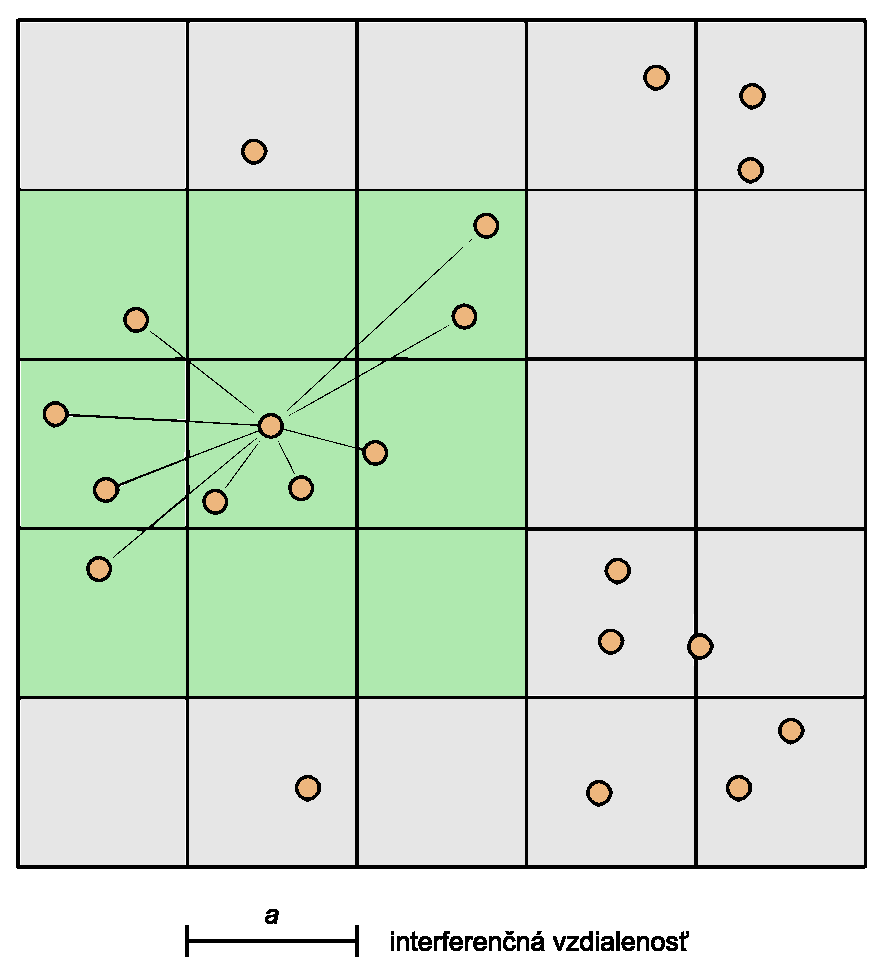
\includegraphics[width=120mm]{figures/channelcontrol_areas}
\caption{Ignorovanie spojení medzi uzlami z kvadrantov, ktorých vzdialenosť presahuje hodnotu interferenčnej vzdialenosti}
\label{fig:channelcontrol_areas}
\end{center}
\end{figure}
\paragraph{Mobility}
\indent Je prirodzené, že každý uzol bude zodpovedný za svoj pohyb po priestore. Teda mobilita zariadení je realizovaná distribuovane v každom uzle. Je riadená modulom \ttfamily Mobility\rmfamily, ktorý je obsiahnutý v štruktúre každého uzla. Aj toho statického, pretože \ttfamily Mobility \rmfamily pridáva k vysielanému rámcu doplňujúce dáta pre \ttfamily ChannelControl\rmfamily, vďaka ktorým je známa poloha prvku a môžu sa prepočítať vzájomné vzdialenosti medzi uzlami. Pre zníženie náročnosti je volaná priamo metóda na objekte \ttfamily ChannelControl\rmfamily. Ušetria sa tým prostriedky na správu ďalších brán, vytváranie nových správ a ich rušenie u~príjemcu. Zásluhou modulu \ttfamily Mobility \rmfamily je aj aktualizovaný pohľad na simulačné pole pri zapnutom GUI počas simulácie. Smer komunikácie medzi \ttfamily ChannelControl \rmfamily a\ttfamily~Mobility \rmfamily modulmi v rôznych uzloch je ilustrovaný na obr.~\ref{fig:topology_mobility}.\\
\begin{figure}[htbp]
\begin{center}
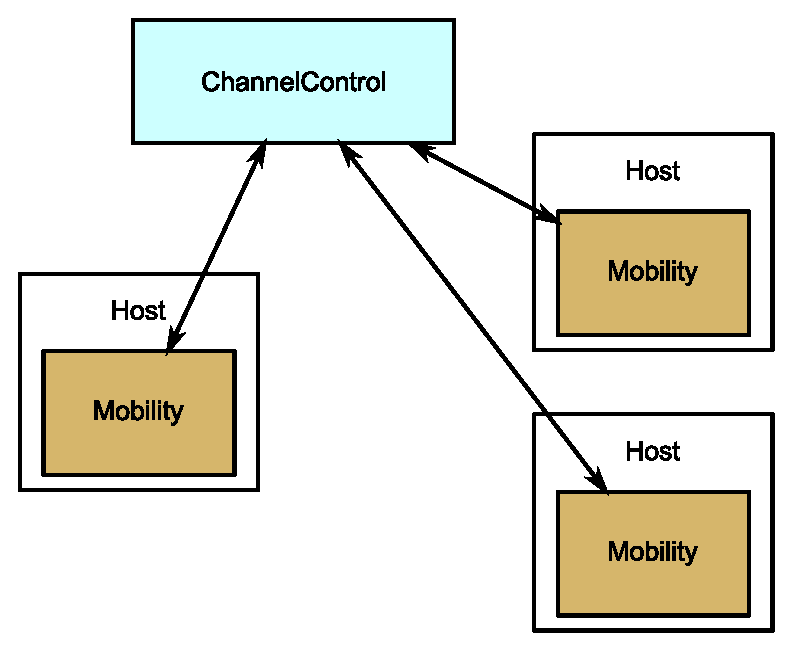
\includegraphics[width=120mm]{figures/topology_mobility}
\caption{Komunikácia medzi modulmi \ttfamily Mobility \rmfamily a \ttfamily ChannelControl\rmfamily}
\label{fig:topology_mobility}
\end{center}
\end{figure}
\paragraph{Blackboard}
\indent Koncept \texttt{Blackboard} sprostredkúva komunikáciu medzi typu od jedného k~mnohým (one-to-all). Je súčasťou každého hostu a vďaka nemu prebieha výmena informácii aj medzi tými vrsvtami, ktoré nemaju spoločný komunikačný kanál. Komunikácia potom funguje spôsobom zverejňovania informácii (publish) na Blackboard a pripísaniu sa k odberu týchto informácii (subscribe). V konečnom dôsledku príjemca má možnosť zistiť, kto bol pôvodcom informácie. Moduly, ktoré sú prihlásené k odberu správ sú upozornené v prípade, že dáta, o ktoré mali záujem, boli sprístupnené alebo aktualizované. V ďalšom kroku ich potom môžu prečítať.\\
\indent Príklad efektívneho použitia tohoto modulu si môžme predstaviť pri bezdrôtovej komunikácii pomocou metódy CSMA-CA, kedy po odoslaní správy sa rádio môže prepnúť do stavu \textit{RX} a túto informáciu zverejní na Blackboard. Vďaka tomu potom povedzme modul, ktorý simuluje energetické zdroje vie, že príkon rádia sa zmenil a zároveň túto informáciu využije aj linková vrstva, ktorá vďaka nej vie, že správa bola odoslaná.\\
\paragraph{Decider}
\indent Modul \texttt{Decider} spracováva informáciu vyslanú fyzickou vrstvou, pomocou použitej modulačnej schémy spočíta hodnoty BER (Bit Error Rate) a prípadne označí bity prijaté s chybou. Tento modul je špeciálne užitočný pri pracovaní s datovými tokmi s premenlivou priepustnosťou (rozdielny bitrate hlavičky a tela - IEEE 802.11) a tým, že je oddelený od ostatných zložiek fyzickej vrstvy umožňuje programátorovi ľahšie aplikovať zmenu použitej modulačnej schémy pri simulácii.\\

\section{Existujúce modely sietí ZigBee a IEEE 802.15.4}
\indent\indent Po ponúknutí vhodných simulačných nástrojov si viacero skupín vybralo pre simuláciu práve protokol IEEE 802.15.4. Dôvody môžu byť rôzne - mobilita prvkov, bezdrôtová komunikácia, jednoduchá implementácia, prípadne analýza mechanizmu GTS. Z uvedených nástrojov vzťahujúcich sa k simulátoru OMNeT++ sú k dispozícii viaceré čiastočné implementácie protokolu IEEE 802.15.4. V krátkosti ich popíšeme na v tejto kapitole.\\
\paragraph{PAWiS (Institute of Computer Technology, Vienna University of Technology)}
\indent Simulátor PAWiS ponúka základ pre linkovú vrstvu ZigBee protokolu. Pri analýze zdrojového kódu tejto vrstvy sa ukázalo, že sa jedná o čiastočný základ MAC vrstvy. V~zjednodušenej podobe zvláda CSMA algoritmus. V kontexte s ostatnými produktami v~rámci daného projektu sa jedná skôr o vedľajší výstup.
\paragraph{MiXiM}
\indent Aj v simulátore MiXiM je pripravená implementácia štandardu IEEE 802.15.4. Táto je totožná s tou z Mobility Framework, je z nej totiž portovaná. Podrobnejšie si ju rozoberieme v nasledujúcom odstavci.
\paragraph{MF (Jérôme Rousselot)}
\indent V Mobility Framework vo verzii 2.0 preview 1 sa objavila v istej podobe naimplementovaná linková vrstva protokolu IEEE 802.15.4. Táto implementácia je čistou implementáciou algoritmu CSMA-CA. Veci ako podpora pre \textit{SLEEP} mód rádia, pre GTS sloty, osirotenie, alebo beacon rámce v nej nie je obsiahnutá. Podoby uvedeného modelu sú dve. Predstavujú implementácie kariet Texas Instruments CC 2420 802.15.4 a Texas Instruments CC 1100 802.15.4, a to pre frekvenčné pásma 868~MHz a 2.4~GHz. Podľa toho sú následne nastavené okrem hodnoty frekvencie nosnej aj veľkosti hlavičiek rámcov, dĺžka SFD (Starting Frame Delimiter), hodnoty viacerých časovačov (napr. ACK timeout).
\subparagraph{MF (Autor)}
\indent Naša predchádzajúca práca venovaná simulácii WSN sietí~\cite{halas03} bola doplnená o jednoduchú implementáciu fyzickej, linkovej a sieťovej vrstvy protokolov ZigBee a~IEEE 802.15.4. Táto implementácia obsiahla procedúry pre vytvorenie siete PAN koordinátorom, správu asociácii a vysielanie beacon rámcov.\\
\indent Tým, že sa autor podieľal na príprave tohoto modelu, bol pôvodne zámer ho rozšíriť a~doplniť chýbajúce procedúry. Okrem toho boli vydané nové verzie štandardov ZigBee a aj IEEE 802.15.4, čo sa tiež odrazilo v snahe reflektovať tieto skutočnosti v novom modeli. Vtedy sa ale ukázal prvý nedostatok prvého produktu. Nízka modularita. Úprava na štandard IEEE 802.15.4b-2006 by si vyžiadala relatívne veľké zásahy. Ďalšie negatívum, bolo zlúčenie modelu fyzickej vrstvy ako je definovaná v dokumente a fyzickej vrstvy ako ju poníma Mobility Framework. Toto pri danej práci nebolo silnou prekážkou, no v prípade, že sa nájde záujemca o použitie modelu vo frameworku MiXiM, ktorý má tendenciu stať sa náhradou za MF, spraví mu taká implementácia fyzickej vrstvy zopár starostí. A ako jednu z posledných vecí, kde by bolo vhodné zmeniť prístup, je komunikácia medzi vrstvami, kde je preposielanie riadiacich inštrukcii riešené cez modul \ttfamily Blackboard\rmfamily. Teraz bude snaha výhradne o~preposielanie správ. \ttfamily Blackboard \rmfamily bude slúžiť na prenos riadiacich a stavových informácii medzi časťou fyzickej vrstvy, ako je k nej pristupované z pohľadu MF a ako časťou fyzickej vrstvy, ako je popísaná v štandarde.

